\documentclass[msthesis.tex]{subfiles}
\def\Arrow{\raisebox{0.3\height}{\scalebox{2}{$\Rightarrow$}}}
\begin{document}

\chapter{Methods}

A classification task  on data from the Human Connectome Project was designed according to the pipeline presented in Fig. \ref{fig:pipeline}.  This pipeline consisted of four major steps. First, the whole brain tractography was first generated on the basis of DWI scans. Second,  a connectome was created and represented in the form of connectivity matrices. Two different feature selection techniques were run for classification of subjects based on the features in the connectivity matrices. Finally, these two techniques were compared based on classification metrics and the features they selected. 

The implementation of this pipeline was scripted in \textit{Python}. The preprocessing of the HCP data to generate tractography was done with the help of \textit{Mrtrix3}.  Data was prepared in a classification ready format using \textit{Pandas} (\cite{pandas_2020}) dataframes. The Maximum Edge Weight Subgraph problem was implemented in \text{Java} based on a modification from \cite{DBLP:journals/corr/LobodaAS16}. The final classification was based on machine learning from \textit{scikit-learn}(\cite{sklearn_2012}). 
\begin{figure}
    \label{fig:pipeline}
     \centering
     \begin{subfigure}[b]{0.4\textwidth}
         \centering
         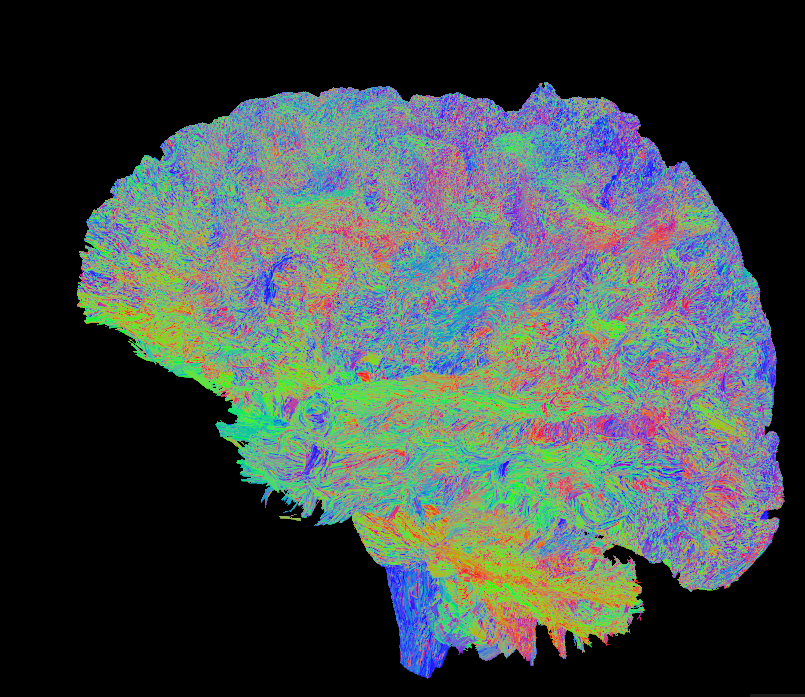
\includegraphics[height=\textwidth,width=\textwidth]{images/tractography.png}
         \caption{$y=x$}
         \label{fig:y equals x}
     \end{subfigure}
     \hfill
    \begin{subfigure}[m]{0.1\textwidth}
        \centering
        \vspace{-5cm}
         \Arrow{}
        \end{subfigure}
    \hfill
     \begin{subfigure}[b]{0.4\textwidth}
         \centering
         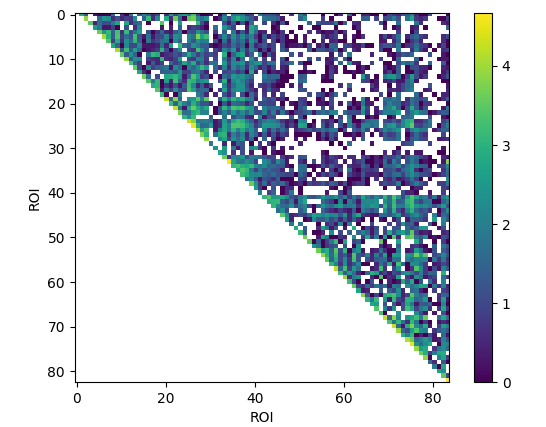
\includegraphics[height =\textwidth,width=\textwidth]{images/connectome_1M.png}
         \caption{$y=3sinx$}
         \label{fig:connectivity_matrix}
        \end{subfigure}
    \vfill
        \begin{subfigure}[b]{0.4\textwidth}
         \centering
         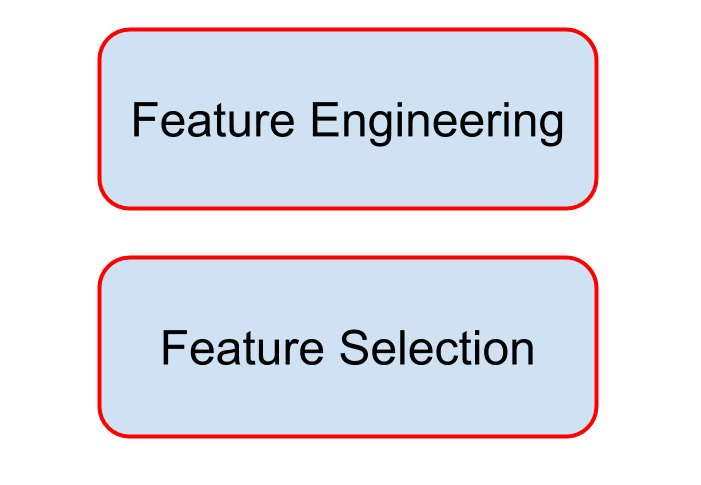
\includegraphics[height =0.8\textwidth,width=\textwidth]{images/Features.png}
         \caption{$y=3sinx$}
         \label{fig:three sin x}
         \end{subfigure}
    \hfill
        \begin{subfigure}[b]{0.4\textwidth}
         \centering
         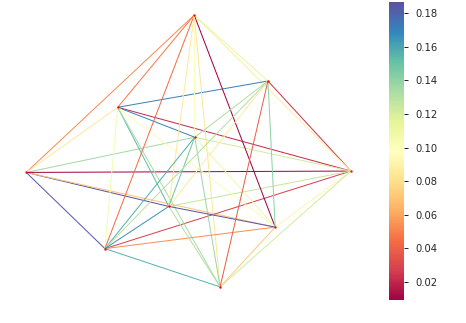
\includegraphics[height =0.8\textwidth,width=\textwidth]{images/mews.png}
         \caption{$y=3sinx$}
         \label{fig:three sin x}
         \end{subfigure}
    \vfill
            \begin{subfigure}[b]{\textwidth}
         \centering
         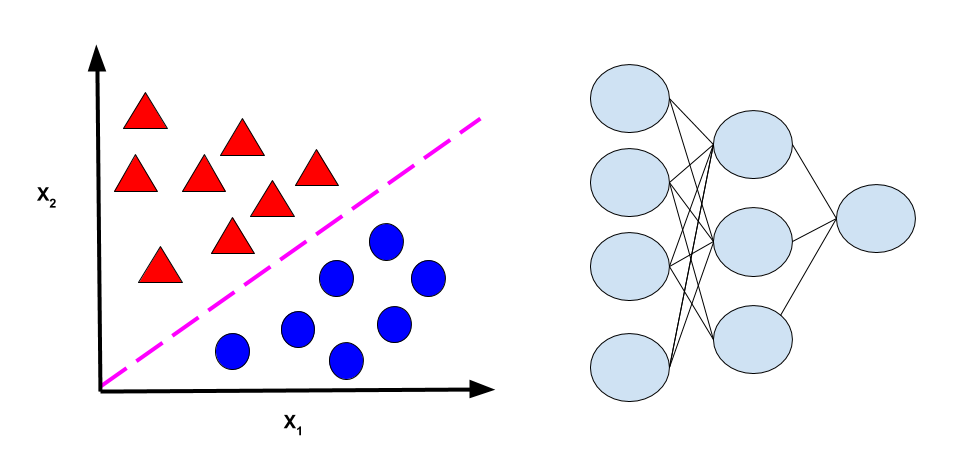
\includegraphics[height =0.5\textwidth,width=\textwidth]{images/classification.png}
         \caption{$y=3sinx$}
         \label{fig:three sin x}
         \end{subfigure}


\end{figure}
\section{Data Acquisition}
\label{sec:acquisition}
Data was acquired for 203 subjects from the s900 release of the HCP (\cite{hcp2015wu}). Out of the total, 101 subjects were female and 102 were male. 83 females and 58 males were aged 26-30 and while the 34 male and 28 females were aged 22-25. The demographic information along with the personality trait labels were obtained from the unrestricted access data available on \href{https://db.humanconnectome.org/}{https://db.humanconnectome.org/}


The structural and diffusion MRI files used for this project were obtained from the repositories containing volumes preprocessed using version 3 preprocessing pipelines of the HCP detailed in (\cite{GLASSER2013105}). A Siemens 3T Skyra system was used used to scan all subjects (starting in August 2012, housed at Washington University, St. Louis). The details of the acquisition protocol are mentioned in \cite{van2012human}.


There were two types of structural data required from the HCP pipeline for each subject in order to proceed with the task of the project. First was the segmentation volume as well as the cortical surface parcellation based on the Desikan Killinay Atlas (\cite{desikan2006automated}, provided as a default in FreeSurfer). Second were the structural scans in undistorted native structural volume space for each subject. This was a T1w volume data in the subject's native space obtained after rigid-body rotation to AC-PC alignment (rigidly aligned to the native axis of MNI space). It was sampled at the same resolution as the diffusion data (1.25 mm isotropic, originally 0.77 mm isotropic). It was important to take into account the images from the subject's native space since it is the one in which the tractography was performed as this space is the best approximation of the subject's physical brain. The parameters of the T1w images are presented in the table \ref{tab:structuralmri}.
\begin{table}[]
    \centering
    \begin{tabular}{|c|c|}
    \hline
         TR (ms) & 2400  \\
    \hline
         TE (ms) & 2.14 \\
    \hline
         T1 (ms) & 1000 \\
    \hline
         Flip angle & 8 deg \\
    \hline
         FOV & 224x224 \\
    \hline
         Voxel Size & 0.77 mm isotropic \\
    \hline
    \end{tabular}
    \caption{Acquisition parameters for the structural image acquisition from the s900 release. }
    \label{tab:structuralmri}
\end{table}

\begin{table}[]
\centering
    \begin{tabular}{|c|c|}
         \hline
         Sequence &  Spin-echo EPI \\
         \hline
         slice thickness & 1.25 mm, 1.25 mm isotropic voxels\\
          \hline
         TR (ms) & 5520  \\
          \hline
         TE (ms) & 89.5 \\
          \hline
         Flip angle & 78 deg \\
          \hline
         Refocusing flip angle & 180 deg \\
          \hline
         FOV & 224x224 \\
          \hline
         Voxel Size & 0.77 mm isotropic \\
          \hline
         b-values & 100,2000 and 3000 s/mm^2\\
          \hline
    \end{tabular}
    \caption{Parameters for the acquisition of the Diffusion MRI data acquired from the HCP.}
    \label{tab:diffusionmripara}
\end{table}
For each subject, four types of files were used. First, the preprocessed diffusion time series file. Second, the brain mask in diffusion space. The other two types were diffusion weighting and diffusion direction for each volume. The important characteristics of the dMRI images is that they obtained in very high resolution (1.25mm isotropic) using a Stejskal-Tanner (monopolar) diffusion encoding scheme as mentioned in section \ref{DWI}. The q-space was sampled by including 3 shells at the b-values presented in table \ref{tab:diffusionmripara} with each gradient table defined by a single b-value acquired once with right-to-left and another in the opposite phase encoding polarities. 


\section{Creating the Connectome}
\begin{figure}
    \centering
    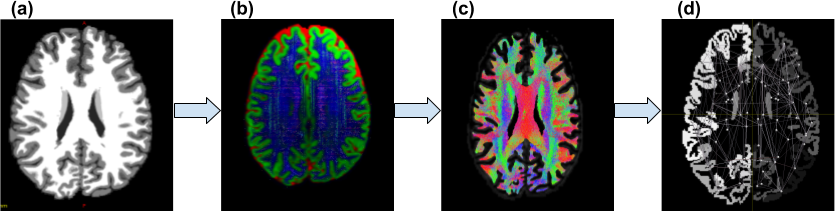
\includegraphics[width=\textwidth]{images/Preprocessing_pipeline.png}
    \caption{Pipeline used to create a connectome for each subject. (a) Five tissue segmented image visualized in grayscale. (b) A slice of a 4D image mapped in 3D using RGB encoding tissue densities, CSF as red, GM as green and WM as blue. (c) Fiber tractography of 1M fibers produced using probabilistic tractography overlaid on an axial slice of the brain. (d) The nodes of the connectome representing ROIs overlaid on an axial slice}
    \label{fig:preproc}
\end{figure}
A connectome is generated on the basis of tractography as explained in section \ref{sec:connectomics}.The pipeline was implemented on the basis of the tutorial on Structural Connectome for Human Connectome from the software package \textbf{\textit{Mrtrix3}}. The preparation of the structural connectivity matrices can be visualized in the figure \ref{fig:preproc} mainly involves three steps which are explained in the following subsections.

\subsection{Structural  and Diffusion image processing}
\label{subsec:struct_diff}

The structural and diffusion images available within the HCP data were used to prepare the data for probabilistic whole-brain tractography (\cite{parker2003framework}). the parcellation image was used to generate a volume delineating locations of the nodes of the connectome for each subject while the T1w image in a subject's native space were used to generate a five-tissue type segmented image.

The default Desikan-Killiany parcellation image as provided by FreeSurfer was converted a nodes image having node numbers starting from 1. FreeSufer's estimates of sub-cortical grey matter structures in the new nodes image was replaced with the estimates from FSL's FIRST tool. 

For each subject, a 5TT segmented was generated on the basis of the structural volume (present in the subject's native space) sampled at the same resolution as the diffusion data (1.25mm isotropic). This allowed mapping of the regions into five tissue types, namely "subcortical white matter (WM)", "WM", "CSF" and optionally "pathological tissue". The segmentation is based on FSL segmentation tools FIRST and FAST.This information about the location of different tissue types makes the tracking based on DWI images suitable for Anatomically constrained tractography.  (\cite{anattractsmith}).

The 5TT image cannot be easily visualized in three dimensions. This problem was solved by estimating the response functions for multi-shell, multi-tissue constrained spherical deconvolution (MSMT-CSD)  based on the algorithm in \cite{jeurissen2014multi}. After obtaining three different files, each consisting of the response functions from the WM, GM and CSF separately, MSMT-CSD is performed to obtain fiber orientation distributions. It generates three different volumes which are then combined to generate a 4D image. In this 4D image, each volume represents the corresponding tissue densities of WM, GM and CSF. The 4D image is then visualized as an RGB image with each volume getting its specific color (Fig. \ref{fig:preproc}(b)). 


\iffalse
The diffusion image was first converted to a non-compressed format. The information about the diffusion gradient encoding was represented in the header of the file, the volume data was made continuous voxel-wise and the data points were converted to a floating point format. 
After this, the mean b=0 image was generated for visualization. The b=0 image serves as a sort of baseline for anatomical reference.

The multi-shell, multi-tissue response function was determined  in order to form Multi-Shell, Multi-tissue spherical deconvolution. 

Atleast three unique b-values are required to estimate three tissue comparments. These 

The deconvolution leads to the formation of a 4 dimensional image in which each 3D volume (as viewed in \comment{part of pipeline figure in preprocessing} is RGB encoded where the cerebrospinal fluid (CSF) is seen in red, the gray matter in green and the white matter in blue. 
\fi

\iffalse
In order to prepare for the tractography, the structural T1w images were preprocessed by Dr. Regina Wehler during the course of her master's thesis. At first the five-tissue-type images were generated using the 5ttgen fsl command. These are segmented 4D images whose fourth dimension represents 5 volumes containing the partial fractions of cortical gray matter, sub-cortical gray matter, white matter, CSF and pathological tissue. 
The input files were converted from the nifti to the mif format using the mrconvert command for the data to be compatible with \textbf{\textit{Mrtrix3}}. Then the 5TT images were generated using the 5ttgen fsl command -nocrop option to keep the images at the size of the original input. 
After obtaining the 5TT images, the segmentation from the original FreeSurfer format were converted to the scheme of the Desikan Killiany Atlas(\cite{desikan2006automated}) which divides the human cerebral brain into gyral based regions of interest.
\fi

\iffalse
\begin{figure}
    \centering
    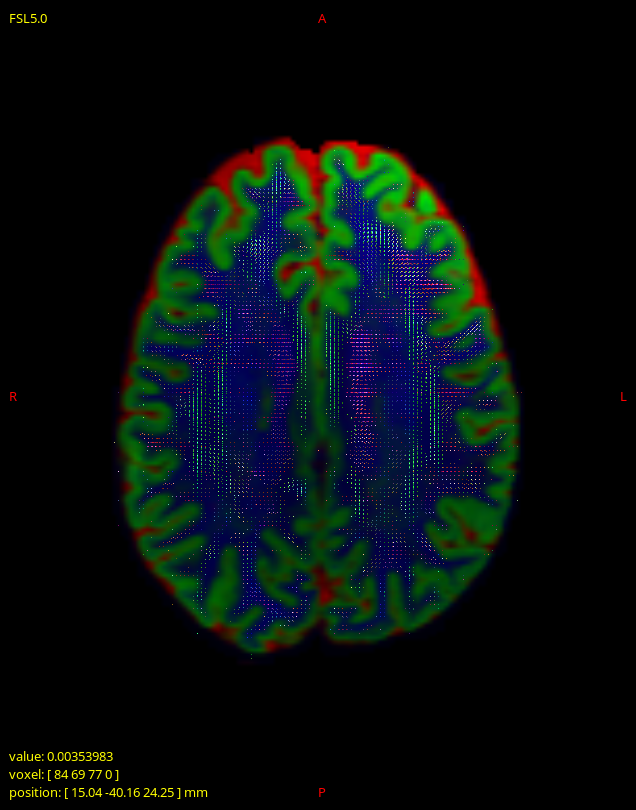
\includegraphics[width=0.5\textwidth]{images/tissueRGB0003.png}
    \caption{Caption}
    \label{fig:tissueRGB}
\end{figure}
\fi
\subsection{Tractography}

Intially, probabilistic  whole-brain tractography of 5M tracts was generated using \textbf{\textit{Mrtrix3}} for all subjects. The streamlines were computed on the basis of the algorithm iFOD2 (\cite{tournier2010improved}). This algorithm uses the fiber orientation Distribution (FOD) image and determines candidate streamline paths (arcs). which have greater FOD amplitudes along them. Then it samples the underlying FOD amplitudes along these arcs. This makes the streamlines more likely to follow paths. Anatomical constraints on the tractography were provided using the five tissue type image. There were other series of constraints imposed in order to make the  tractography more informed. 

The seed points were dynamically determined using the Spherical-deconvolution informed filtering (SIFT) model \cite{smith2013sift} of the white matter fODFs. The cutoff value of 0.06 was set for FOD amplitude for terminating tracks. The maximum length of streamlines was set at 250 mm (200 times the voxel size) when the voxel size is 1.25mm.The tracking along a streamline was truncated if the fiber terminates at poor structural, then  retracking is performed. The streamlines were cropped whenever as the streamlines cross the grey matter-white matter interface. 

The \textit{tcksift} command was used to downsample the tractography from 5M fibers to 1M fibers to preserve the most biologically relevant fibers using the SIFT algorithm (\cite{smith2013sift}). This provides more meaningful estimates of the structural connection density and also reduced the memory requirements. 
\iffalse
\begin{figure}
    \centering
    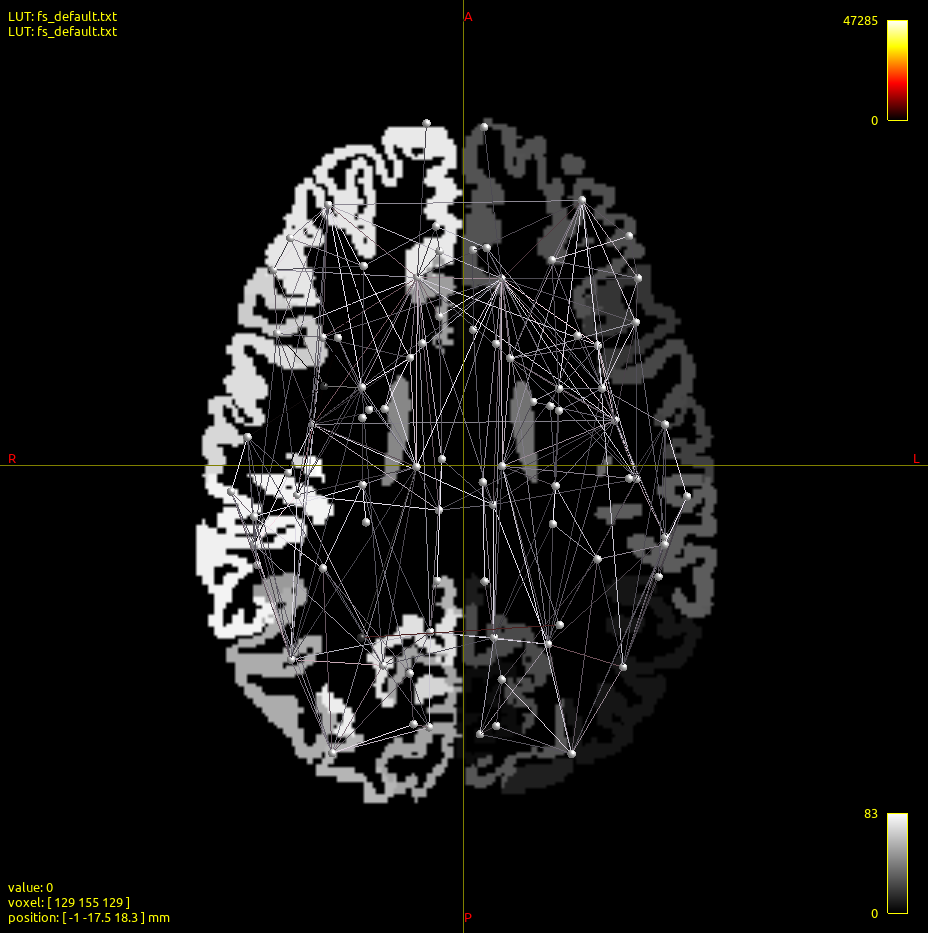
\includegraphics[width=0.8\textwidth]{images/connectome.png}
    \caption{Caption}
    \label{fig:connectome_vis}
\end{figure}
\fi
\subsection{Connectome Generation}

The connectome can be represented in the form of a graph as mentioned in section \ref{sec:connectomics}. After obtaining the streamline file and a parcellation image representing the subject specific node locations of the connectome, the connectome matrix was obtained in a .csv format. It was generated from the 1M fiber tractography using 84 relevant grey matter parcellations (in \textit{\textbf{Mrtrix3}}) from the default FreeSurfer segementation specified by the Desikan Killiany Atlas. 

Using different parameter settings from the \textit{tck2connectome} command three types of features  were extracted. The mean fractional anisotropy (or mean FA, equation \ref{eq:meanFA}), of the streamlines that connect the two regions, the mean streamline length and number of streamlines between any two regions. The visualization can be seen in the figure \ref{fig:connectivity_matrix}. The connectome is represented in an upper triangular matrix format (.csv file) that 84x84, considering that the connections between two ROIs are symmetric.

\iffalse
In the Fig. it can be seen that there is a need to decipher the streamlines which are terminating in the specified regions of interest
\fi
\section{Feature representation}
Once the connectivity matrices for all the 201 subjects were computed and encoded in the format of a .csv file, a \textit{pandas} dataframe was prepared in order to be prepared to fit into the classifier. Each row represented the data for an individual subject. Each column represented the connection between any two brain regions i.e. features in one cell of the connectivity matrix. The exact structure varied according to the feature selection techniques employed.

The whole experiment was divided into two types of experiment. The first was in the form of a baseline where the feature selection was based on statistical scores such as fscores, t-tests and pearson correlation coefficients. This type of feature selection was termed as the 'baseline' experiments set. The second approach, added another layer to the first approach with the incorporation of MEWS problem to reduce the graphs into smaller subgraphs explained in the later section.
\subsection{Exclusion of self loops}
Self loops are considered the connections from the brain regions to themselves. On the basis of performance of the classifiers it was seen that without the self loops the performance the classifiers still perform almost similarly.

To see the difference in between the classification accuracies, a paired sample t-test was conducted. In this t-test the paired samples are the classification metrics in the dataframe including the self loops and excluding them. The null hypothesis of this two-sided t-test was that the average of a particular classification metric on the basis of one feature (such as mean FA, mean streamline length etc.) with respect to five different personality traits was identical. The null hypothesis could not be rejected because for the test data, the p-values of these t-tests was high and hence not corresponding to any statistical significance. 
\iffalse
avg mean FA for all self loops(along all subjects in training data) 0.36
avg mean FA for all the other areas without the self loops (across all the subjects) is 0.345 (avg)
max avg mean FA in the range is 0.66 (in one connection avg along all subjects)
\fi

\subsubsection{Statistical Coefficients}

Statistical coefficients were determiend to be one of the most important feature filter methods in the analysis.
The fscore used in the analysis is used to measure how well the particular feature distinguishes between the two classes labelled as 1 and 2. It has the expression according to the equation \ref{eq:fscores}. The fscores served as feature filtering step for the baseline experiments as they were used by dividing the f-score distribution into percentiles and then choosing the percentage of features we want in the specified top percentile. However, for the solver based experiments the fscores for each feature was (numerically) low which made the MIP problem hard to run computationally. Even multiplying the f-scores with an order of $10^3$ was not useful since the standard deviation of the f-scores was not too high (insert the standard deviation). 

Similarly, an independent sample t-test was applied to consider the training subjects and the test subjects as independent samples, with the null-hypothesis that the means of the given feature for the two samples are identical i.e. $\overline{x_{1}} - \overline{x_{2}} = 0$. This feature selection was in fact quite useful for the feature selection in the baseline experiments. The p-value of the t-test could be divided into percentile distributions and the top percentiles could be chosen accordingly. However, for the solver based experiments this selection did not work well due to computational effort. 

The pearson correlation coefficient in fact did work because it considers the linear nature of the personality trait coefficients. This type of feature selection is well reported in literature for Neuroimaging data considering continuous variables. It performed well for the baseline experiments as well as the solver based feature selection. For both the cases the absolute value of the pearson correlation coefficient was taken because only the correlation was important, whether it is positive or negative correlation was not a matter of concern for the analysis.

The f-score and the t-test were based on the binarization of the target variables according to the median values of the feature from the training set, this might lead to information loss and hence their lower numerical values. 

\subsection{Feature selection} 
There were two types of feature selection techniques used before classification. The first represents a classical feature selection technique based on statistical coefficients while the second is based on extracting a subgraph. The Maximum edge weight subgraph techniques is based on exploiting the topological nature between the subnetworks while the first approach is based purely on numerical artefacts. To hypothesize with the connecitonist view of the brain, sugraph technique shall give rise to more interpretable results as it is based on the fact that certain brain connections are more important than others when it comes to classifying a particular type of label. The motivation to implement subgraph extraction methods is the fact that analyzing the inter-subject differences at the subnetwork level is much more easier than analyzing dense subgraph of whole brain connectivity. 

\subsubsection{Statistical analysis}
% Question: which one do we report? Solver was working only with the pearson correlation coefficient.
Three different metrics were used to filter the features. Namely, pearson correlation coefficient, f-scores and the p-value of the t-test. The pearson correlation coefficient for the continuous values of the different personality traits, while the f-scores and t-test calculations were based on the conversion of the continuous variables into classes according to the section \ref{sec:label_preparation}. These metrics were then used to rank the features.

The pearson correlation coefficient was computed between the values of the feature for the training subjects and their corresponding personality trait values. It was a trial to capture the linear relationship between the value of the structural brain connection and the outcome label. Using the numerical coefficients the features were selected on basis of top k\% numerical values.

The fscore based selection was done by computing the fscore between thhe feature values for the training set and thresholded values of the target variables according to the medinan of the training data labels. These scores were then ranked using percentiles and fed to the classifier. 

The t-test carried out was an independent two sample t-test with the null hypothesis that the training subjects come from the same population and have the same average of the numerical feature values. It was processed in a different manner as compared to the first two metrics, on the basis of the classes the training data was divided into two groups, one belonging to class 0 and the other belonging to class 1. Then the t-test was computed for each feature and the features which gave low p-values (insert threshold) were selected. 
\subsubsection{Maximum Edge Weighted Subgraph}
\labe{method:MEWS}
The input graphs implemented for the use-case of this thesis consisted of 84 nodes defined by the cortical parcellations based on the Desikan Killiany Atlas. The edges represent the properties of the connections between these nodes. 

In this approach, there was one graph created for all subjects to get a generalized representation of connection strengths. First, from the calculation of the statistical coefficients of the brain connections (each feature) with respect to the target labels was determined. These coefficient values (one value for one connection and all subjects in the training set) formed the edge weights of the graph given as an input to the solver. Once the input graph was formed it was filtered to introduce sparsity. This sparsity was introduced using two constraint. The first being that the absolute value of the edge weights shall not be zero and that the edges will be fed into the solver if and only if the tractography of each subject contains atleast one streamline between the two nodes. 

The edge weights represented the Pearson correlation coefficient (computed on the basis of the training data) of the individual feature values with the continuous personality trait variable. 

The subgraph was meant to represent the most discriminative connections  Based on the implementation by the authors, \cite{DBLP:journals/corr/LobodaAS16}, the two major components are maximizing the function (\ref{eq:sumfun}) and imposing constraints for the subgraph to be connected. The connectedness contraints are implemented using a Mixed Integer Programming formulation. 

\begin{itemize}
 \item $m \in [1,84]$ specifying the number of nodes to be preserved in the output graph
\end{itemize}
Using these variables a set of equations can represent the structure of the subgraph:
\begin{align}
    \label{eq:sum_constraints}
    \sum_{v=1}^{V} y_v = m        &&  \forall v \in V
\end{align}
According to  equation \ref{eq:w_e}, an edge can be present in the subgraph only if both the vertices connecting the edge are included in the subgraph. Equation\ref{eq:sum_constraints} ensures that the specified number of nodes $m$ are preserved. 


\section{Supervised Classification}

\subsection{Label Preparation}
\label{sec:label_preparation}
There were two different ways in which the continuous personality traits were converted into categorical variables. 
\begin{enumerate}
    \item All the values of a particular trait above or equal to the median value get assigned as 1. 
    \item Split the variable's distributions into three quantiles containing 1/3 of the data in terms of frequency. 
\end{enumerate}

\subsection{Classification}
\begin{itemize}
    \item Support Vector Machines
    \item Random Forests

\end{itemize}




\end{document}

